% Usar el tipo de documento: Artículo científico.
\documentclass[11pt,a4paper]{article}

% Cargar mensajes en español.
\usepackage[spanish]{babel}

% Usar codificación utf-8 para acentos y otros.
\usepackage[utf8]{inputenc}
\usepackage[T1]{fontenc}
\usepackage{lmodern}

%Dimensiones de los márgenes.
%\usepackage[margin=1.5cm]{geometry}

% Insertar porciones de código
\usepackage{listings}

% Comenzar párrafos con separación no indentación.
\usepackage{parskip}
%enlaces
\usepackage{hyperref}
% Usar gráficos
\usepackage{graphicx}
\usepackage{caption}
\usepackage{subcaption}
%
% Usar contenedores flotantes para figuras.
\usepackage{float}

% Carpeta de las imágenes.
%\graphicspath{{img/}}



%Gummi|065|=)
\title{\textbf{Deeper. Bienvenido al futuro}}
\author{rodrigo.arias@udc.es}
\date{}




\begin{document}

\maketitle

\section{Introducción}
\subsection{Expectantes}

Al fin y al cabo un videojuego es la realización más atractiva que uno pudiera 
plantearse al producir gráficos en un ordenador.

Introduce al sujeto en una nueva realidad, provocando que experimente nuevas 
situaciones que han sido cuidadosamente elaboradas. Con el mero propósito de 
causar una sensación sin igual, sin precedentes.

Las cualidades son bien conocidas. Lugares exóticos que no podrían ocurrir en el 
mundo actual. Al menos no en nuestra época. Un sueño donde somos conscientes.  

A todos nos encanta viajar. Experimentar las costumbres de otros lugares.  
Olvidarnos por un segundo de nuestra pequeña burbujita y emprender una aventura.  
Sin conocer el final. Expectantes.

Entonces la modernidad de una época, junto a la intriga más profunda, trastoca 
el significado de la antigua palabra para incluirla en el eje temporal. Que 
ocurriría si pudiesemos hacerlo. Viajar en el tiempo.

Paradojas, dicen los expertos. Pero eso no sacia nuestra curiosidad. No nos 
detiene. Veámoslo con nuestros propios ojos.

\subsection{La máquina}

Es preciso una máquina. Un dispositivo no mucho más grande que una caja donde 
cabe una persona. Un temporizador permite ponerla en funcionamiento de forma programada.

El funcionamiento es bastante sencillo. Aunque sus consecuencias no lo son 
tanto.

Primero activa el temporizador para programar el encendido de la máquina.  
Debes anotar el momento exacto en el que la máquina será activada. Llamaremos a 
este instante el momento A. Asegúrate de que tienes tiempo suficiente para salir 
de ahí, pues no quisieras encontrarte con quien tú sabes.



Aléjate, y realiza las tareas que desees mientras dejas que la máquina se 
encienda sola. Cuando estés listo, prepárate para entrar en la misma. Anota el 
momento exacto en el que entras en la máquina. Este será el momento B.

La máquina te llevará de vuelta al momento A. En ese instante existirán dos 
versiones de tí mismo.

Mantén especial cuidado en no modificar la conducta que has realizado antes de 
entrar en la máquina. Si lo haces, las consecuencias son inciertas. 

\subsection{Consecuencias}

Y entonces, ¿que ocurriría? El juego permite realizar viajes en el tiempo y 
observar los efectos que provoca. Permite aprovechar las ventajas de viajar en 
el tiempo, para poder resolver una serie de escenas.

En cada escena deberás alcanzar un lugar determinado para continuar. Para ello, 
utiliza los objetos que encuentres, y usa tu imaginación e ingenio para resolver 
el rompecabezas.

\subsection{Mecanismo de tiempo}
El tiempo que conocemos transcurre de forma lineal. Todo suceso que se produce, 
es debido a unas causas posteriores.

La introducción de una máquina capaz de teletrasportar a una persona al pasado 
lo cambia todo.

Cada vez que viajas en el tiempo, el eje temporal se divide en dos partes. Para 
realizar viajes temporales, es adecuado incluir un número que identifica a una 
persona en un eje temporal concreto.

Veamos un ejemplo. Al comienzo, tu número es el 1, y aún no has realizado ningún 
viaje temporal. Entonces decides probar a viajar en el tiempo. Para ello has de 
encender una máquina.

Cuando la acciones, esta quedará programada para encenderse, y tras un rato se 
encenderá. Después de programarla te diriges a la cafetería y te tomas un café.  
Luego, irás a trabajar como todos los días, donde pasarás el resto del día, 
hasta la noche.

Al volver, la máquina ya se encuentra encendida, y puedes usarla. Al meterte 
dentro, la máquina te transporta al pasado, en el momento en el que te 
encontrabas desayunando en la cafetería. Ahora eres el numero 2. Entonces te 
diriges a la cafetería y te sientas muy alejado de ti.

Mientras desayunabas, no pensabas en absoluto que tu mismo estuvieras ahí en la 
cafetería, pues fue una decisión que tomaste despues. El efecto, aparecer en la 
cafetería, ocurre antes de las causas. Y es algo que tendrás que tener en cuenta 
para poder viajar en el tiempo.

En el juego, puedes acercarte tanto como quieras a tu doble, pero no puedes 
tocarlo. Si lo haces, un mecanismo de protección te echará fuera del eje 
temporal, y te devolverá al comienzo del nivel.

Veamos que más puede ocurrir. Te levantas, y vas a donde habías aparcado tu 
coche, y rompes todos los cristales. Es algo que no ocurrió en el pasado, y por 
lo tanto, estás alterando los hechos. Cuando vayas a subirte para ir al trabajo, 
el estado del coche, ya no será el mismo. Esto no debe ocurrir, ya que estarías 
cambiando el transcurso del pasado. El juego dispone de un mecanismo, que 
protege a todos los objetos. Si detecta que uno no se encuentra en el mismo 
estado, te devuelve al comienzo.

Estos problemas, se pueden evitar, si sigues las reglas de viajes temporales de 
Shane Carruth, adaptadas a este juego:
\begin{enumerate}
\item Planifica tus viajes primero.
\item No toques la máquina después de salir de ella, tu doble la usará.
\item Cuando compartas el tiempo con tu doble, mantente alejado de él.
\item Preocúpate primero por tí. El presente es el único momento que tiene 
sentido.
\item No seas curioso con lo que te rodea.
\end{enumerate}

\section{Historia}

No existe un futuro establecido. El personaje aparece en un escenario sin saber 
muy bien ni el objetivo, ni lo que debe hacer. Pero poco a poco descubre que las 
máquinas que le proporcionan los viajes en el tiempo para resolver el nivel, son 
las mismas que lo transportan al siguiente.

El juego describe una historia invertida. Un viaje en el tiempo, pero al pasado.  
Cada nivel es un paso más en la historia. Este hecho es el que le pone nombre al 
juego.

El creador de la máquina, ya era muy consciente de lo que ocurriría si encendía 
la máquina por primera vez. Los posibles viajes desde el futuro eran 
impredecibles.  De modo que decidió elaborar una serie de puzzles, de forma que 
sólo él pudiera volver al pasado, al momento en el que construía la máquina.

Todo un ingenioso mecanismo que impedía que se pudiera alcanzar el momento cero, 
en el caso en el que algo saliera mal. Sólo entonces se podría impedir a sí 
mismo la activación de las máquinas iniciales.

Mientras se cubría las espaldas, no se daba cuenta de lo importante que 
resultaría mantenerse con vida. Sólo él conocía los complicados laberintos, que 
permitían el control ilimitado de las máquinas.

Pues tan sólo tres máquinas modulares, permiten realizar infinidad de copias, 
realizando viajes consecutivos al pasado, viajando con las dos máquinas 
restantes. El mundo que se observa en el juego, no es más que la misma máquina, 
colocada por el creador en lugares determinados en un tiempo concreto.

Tu objetivo es impedir la construcción de las máquinas, y para ello has de 
resolver el complejo laberinto que el creador había ideado. El por desgracia, ya 
no puede hacerlo, ni ningún otro ser vivo. Los viajes en el tiempo pueden tener 
consecuencias desastrosas.

\subsection{Diagramas}

Para la representación de los viajes en el tiempo, se ha empleado una versión de 
los diagramas de Feynman para la evolución de las partículas con el tiempo. Pero 
adaptados a los viajes temporales. En el eje horizontal se representa el tiempo, 
y en el vertical una posición del espacio.

\begin{figure}[htp]
\centering
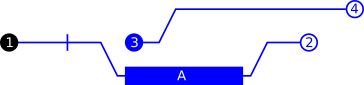
\includegraphics{cronograma1.png}
\caption{Diagrama del primer nivel}
\label{}
\end{figure}

Se recomienda el uso de este tipo de diagramas para la resolución de los
niveles. Sobre todo aquellos que impliquen varios viajes en el tiempo.

En el punto 1, el personaje se encuentra frente a una máquina apagada. La marca 
vertical indica que programa la máquina. Luego se dirige a otro lugar, y acciona 
la palanca A. La mantiene accionada un tiempo, y luego vuelve a la máquina, en 
el punto 2. Entonces viaja al pasado (hacia la izquierda) hasta el momento en el 
que se encendió la máquina, el punto 3. Un poco después de haberla programado 
(la línea vertical). Entonces emplea la plataforma activada por la palanca para 
llegar al punto 4, donde se finaliza el nivel.

\section{Desarrollo 2D}
\subsection{Diseño}

El juego está diseñado por partes más o menos conceptuales.  A continuación se 
mencionan las más importantes del juego.

\subsubsection{SpriteT}

Esta clase, permite añadir a un objeto la representación del tiempo, de la 
posición, velocidad y aceleración. Junto con la clase Gravity, que simula el 
efecto de la gravedad, permiten elaborar los movimientos del personaje. Los 
objetos que deseen obtener esta característica, tan sólo han de heredar esta 
clase.

Es importante mencionar que los objetos mantienen una posición absoluta.  
Empleando el eje cartesiano habitual (X positivo hacia la derecha e Y positivo 
hacia arriba). Sin embargo en pygame el eje Y se encuentra invertido, por lo que 
se ajusta antes de colocarse en la escena.

\subsubsection{Machine}

La máquina es uno de los objetos más complejos. La parte más destacada quizás 
sea su control de las incoherencias. Esto es, una acción que se produce en el 
presente, y que modifica un estado del pasado.

Cuando la máquina detecta esta clase de problemas, efectúa un aviso de 
emergencia que detiene el transcurso del juego y reinicia el nivel.

Por otra parte, las máquinas han sido cuidadosamente elegidas, para que se 
bloqueen en el caso de ser utilizadas. Los bloqueos sirven para prevenir 
incoherencias. Se ha tratado de reducir los bloqueos al mínimo, para que el 
jugador tenga la máxima libertad de elección.

Cuando una máquina se enciende, y a continuación se utiliza, se retrocede al 
pasado, y la máquina queda bloqueada, de forma que sólo el personaje que la 
empleó en su momento, pueda hacerlo. Los demás jugadores no pueden alterarla.

Sin embargo, las máquinas que hayan sido encendidas, pero no usadas, no son 
bloqueadas, permitiendo su uso incluso tras haber viajado en el tiempo.

\subsubsection{Boy}

El personaje está representado por la clase Boy. Se emplea esta clase para el 
personaje que está activo, el que recibe los eventos del teclado y reacciona en 
tiempo real. Y también para los duplicados que realizarán acciones del pasado de 
forma programada.

Emplea las propiedades de SpriteT y Gravity. Además es quien guía la cámara, 
cuando es el personaje activo.

\subsubsection{Clonaciones}

Todos los objetos del mundo (en el juego), implementan los métodos clone y 
restore. Estos permiten obtener toda la información relevante del objeto, y 
restaurarla en el futuro (en realidad en el pasado) respectivamente.

Son muy importantes para poder volver a un punto determinado del pasado, y 
colocar todo objeto en su lugar y en el mismo estado en el que se encontraba.

\subsubsection{Eventos}

Todos los objetos del juego se pueden comunicar entre ellos empleando un sistema 
de mensajes y eventos. EventDaemon recoge los eventos producidos por los 
objetos, y los envía a su destino. Esto es:

Eventos generados por el personaje, como realizar la acción. Que es un evento 
puntual, por lo que se colisiona al personaje y se envía a todos los objetos 
involucrados de forma ordenada. Una vez que el evento es atendido, ya no se 
continúa enviando a ningún otro objeto.

Eventos dirigidos, que son enviados al objeto destino, ya predefinido.

Eventos de teclado, recogidos por EventControl, que son dirigidos al personaje 
activo.

\subsubsection{ObjectManager}

Todos los objetos son registrados por OM (Object Manager). De forma que para 
realizar una actualización de fotograma, secuencialmente va ejecutando el método 
update de los objetos.

Además gestiona las colisiones del personaje con paredes o suelo, y con otros 
objetos.

Para poder depurar el juego, a mayores se incluye en cada objeto un 
identificador numérico, que es asignado por OM, de forma secuencial.

\subsubsection{Camera}
Dado que el personaje activo recibe el seguimiento de la vista del observador, 
todos los objetos dependen de su posición.

Para ello se ha ideado el mecanismo de cámara, que actualiza un valor de 
desplazamiento conforme a la posición del jugador.

Luego, los objetos piden a la cámara su posición en pantalla, donde se 
dibujarán.

De esta forma, la cámara puede cambiar el objeto al que sigue, y el resto de 
objetos, actualizarán sus posiciones en pantalla de acuerdo con la nueva 
información.

\subsubsection{Grabaciones}

Recording es la clase encargada de ir almacenando las teclas que presionas 
mientras juegas, y que son enviadas al jugador activo.

Cuando viajas al pasado, la grabación se pone en marcha, y comienza a repetir 
las mismas pulsaciones que habías hecho entonces sobre tu personaje, de forma 
que actúa exactamente igual que como tú lo hiciste.

Por otra parte, se crea otro personaje nuevo, y se pone en marcha una nueva 
grabación, que captará los eventos de teclado que acciones.

\subsubsection{SVT}

La clase SVT (Sistema de Viajes Temporales) es el centro de control del juego.  
Recibe todos los eventos de máquinas y personajes, y realiza los viajes en el 
tiempo oportunos. Esta clase controla el tiempo absoluto, y el tiempo relativo.

El tiempo absoluto es el tiempo en el mundo real, que es creciente y nunca 
retrocede. El tiempo relativo es el que se representa en el juego, y puede 
cambiar al viajar en el tiempo.

Cada máquina dispone del momento exacto en el que se encendió. De forma que al 
accionarla para retroceder al pasado, se calcula la diferencia con el momento 
actual.

Entonces SVT ha de cambiar la hora del juego, y colocarla en el momento en el 
que la máquina se enciende. Esto supone decrementar el tiempo relativo, 
actualizar el tiempo de todos los objetos, recalcular cuales estaban o no en la 
escena, y reproducir las grabaciones oportunas, entre otras acciones.

\subsubsection{Level}
Implementa una clase abstracta para el desarrollo de los niveles. Cada nivel 
tiene su SVT, EventDaemon y OM. De forma que se manejan conjuntamente en esta 
clase. Luego cada nivel concreto sólo ha de añadir las diferentes 
configuraciones de objetos a OM.

\subsubsection{GameLogic}

Implementa todo el juego. Se encarga de las escenas, como la de muerte o 
incoherencia, y el avance de los niveles.

Cada nivel informa a GameLogic cuando ha de colocar el siguiente nivel. Los 
niveles se mantienen en una pila, en la que se sobreponen las escenas de 
mensajes como SceneFailure.

Cuando ya no quedan más niveles el juego se ha completado.

\subsection{Limitaciones}
El reto del juego era comprender cómo funcionan los viajes en el tiempo, y que 
implicaciones tendrían.

A lo largo del desarrollo se han ido descubriendo problemas, y se han tratado de 
solucionar, respetando un diseño limpio. Sin embargo, dada la gran complejidad 
que conlleva viajar al pasado, este diseño no es realmente sencillo.

Dado el carácter evolutivo que se ha planteado, quizás el método más apropiado 
para continuar el desarrollo es el de la utilización de prototipos. De forma que 
resulta beneficioso descartar algunas partes, y reescribirlas de una forma más 
sencilla.

\section{Niveles}

El juego está constituído de varios niveles. Cada uno tiene una complejidad 
mayor al anterior.

Todos comparten unas características comunes. Una máquina activa es el punto de 
partida del personaje. Sale de la máquina de comienzo.

Luego realiza las acciones que le llevan al lugar de la máquina de fin, que le 
permite viajar a siguiente nivel.

Se puede observar que cada máquina proporciona una conexión con el siguiente 
nivel. De hecho, la historia del juego está muy relacionada con cómo se 
resuelven lo niveles.

La máquina de comienzo no se puede usar en ningún momento, ya que está 
bloqueada. Dado que será usada en el futuro para llegar al nivel actual.

\subsection{Palancas}
Las palancas proporcionan una forma de interactuar con el entorno. Actúan como 
pulsadores, de forma que al soltarlas o al alejarse vuelven a la posición 
original.

Esta propiedad fuerza a que para mantener los efectos de la palanca durante un 
intervalo, sea necesario mantenerla durante ese intervalo.


\begin{figure}[h]
\centering
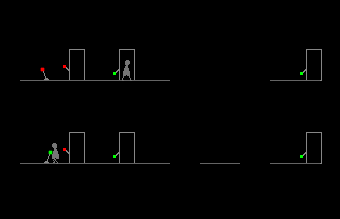
\includegraphics[scale=0.8]{level1.png}
\caption{Dos fotogramas del primer nivel}
\label{}
\end{figure}


\end{document}
